\begin{center}
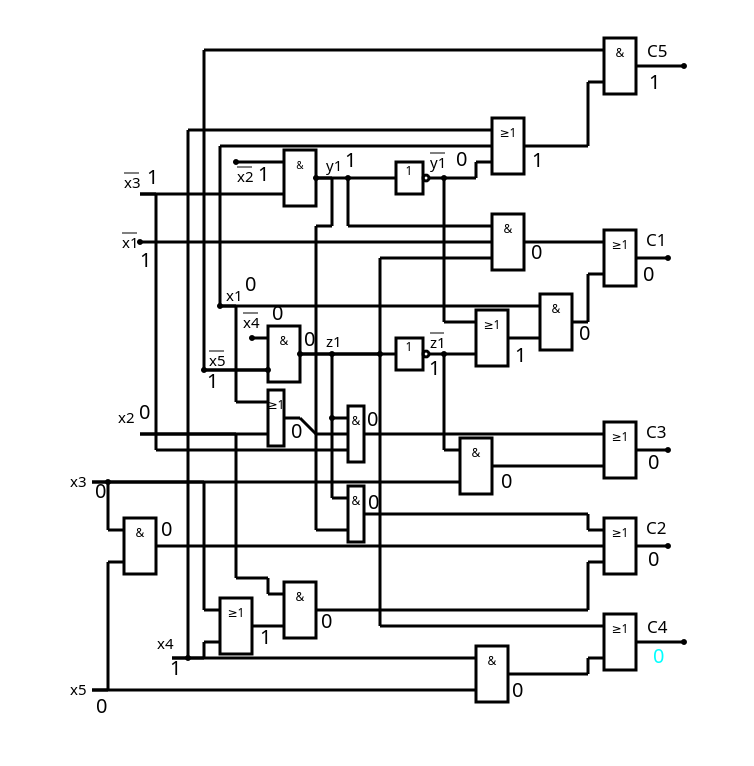
\includegraphics[width=\linewidth]{imgs/part2/circuit-C1-C5_boolean_basis.png}
\end{center}
Задержка многовыходной схемы определяется в отношении каждого выхода: $T_{C_1}=5\tau, T_{C_2}=3\tau, T_{C_3}=4\tau, T_{C_4}=2\tau, T_{C_5}=4\tau$ \\и всей схемы в целом: $T= max (T_{C_2}, T_{C_2}, T_{C_3}, T_{C_4}, T_{C_5})= 5\tau.$